\documentclass[a4paper,oneside]{memoir}
\usepackage[margin=3cm]{geometry}
\usepackage[english]{babel}
\usepackage[utf8]{inputenc}
\usepackage[T1]{fontenc}
\usepackage{amsmath}
\usepackage{graphicx}
\usepackage{amssymb}
\usepackage{booktabs}
\usepackage{fancyhdr}
\usepackage{kpfonts}
\usepackage{booktabs}
\usepackage{gensymb}
\usepackage{float}
\usepackage{bm}					% Tilader matematik skrevet med fed skrift.
\usepackage{color}
\usepackage{fancyvrb}
\usepackage{lastpage}
\usepackage{pgf,tikz,pgfplots}
\usepackage{mathrsfs}
\usepackage{lipsum}
\usetikzlibrary{arrows}
\usepackage{lipsum}
\usepackage{listings}
\lstset
{
	language=[LaTeX]TeX,
	breaklines=true,
	basicstyle=\scriptsize,
	keywordstyle=\color{blue},
	identifierstyle=\color{magenta},
}
\usepackage[normalem]{ulem}
\usepackage{microtype}
\renewcommand{\baselinestretch}{1.2}
\usepackage[numbered,framed]{matlab-prettifier}
\fancypagestyle{firststyle}
{\fancyhf{}
	\fancyhead[R]{Aarhus University
	}
	\fancyhead[L]{PPNM}
	\fancyfoot[C]{\footnotesize Page \thepage\ of \pageref{LastPage}}
	\renewcommand{\headrulewidth}{1pt}}
\pagestyle{fancy}
\usepackage[bottom]{footmisc}
\fancyhf{} % clear all header and footer fields
\fancyfoot[C]{\footnotesize Side \thepage\ af \pageref{LastPage}}
\renewcommand{\headrulewidth}{0pt}
\newcommand{\N}{\mathbb{N}}
\newcommand{\Z}{\mathbb{Z}}
\newcommand{\Q}{\mathbb{Q}}
\newcommand{\R}{\mathbb{R}}
\newcommand{\C}{\mathbb{C}}
\newcommand{\F}{\mathbb{F}}
\newcommand{\V}{\mathcal{V}}
\newcommand{\eq}[1]{\begin{align*}#1\end{align*}}
\newcommand{\pmat}[4]{\begin{pmatrix} #1 & #2 \\ #3 & #4 \end{pmatrix}}
\newcommand{\pvec}[4]{\begin{pmatrix} #1   \\ #2 \\ #3 \\ #4\end{pmatrix}}
\usepackage[hidelinks]{hyperref}
\pgfplotsset{compat=1.15}
\counterwithout{section}{chapter}
\counterwithout{figure}{chapter}
\counterwithout{figure}{section}
\maxtocdepth{subsection}
\setlength{\parindent}{0pt}



% VEKTORKOMMANDOER
\renewcommand{\vec}[1]{\bm{\mathrm{#1}}}						% Standard vektor.
\newcommand{\uvec}[1]{\hat{\bm{\mathrm{#1}}}}					% Enhedsvektor.
\newcommand{\scalarprod}{\bm{\cdot}}							% Skalarprodukt.
\newcommand{\innerprod}[2]{\left\langle #1,#2 \right\rangle}	% Indre produkt.
\newcommand{\norm}[1]{\left\lVert#1\right\rVert}				% Norm.
\newcommand{\abs}[1]{\left\lvert #1 \right\rvert}				% Absolut værdi.

%\addto{\captionsdanish}{\renewcommand{\abstractname}{Resumé}}
\begin{document}

	\author{Martin Mikkelsen  \\
		--201706771-- \\ }
	\title{A brief introduction to the exponential function}
	\maketitle

	%\addcontentsline{toc}{section}{Resumé}


	\thispagestyle{firststyle}

This is a brief introduction to the exponential function. In mathematics, an exponential function is a function of the form
\begin{equation} \label{def}
  f(x)=ab^x,
\end{equation}
where $b$ is a positive real number, and the argument $x$  occurs as the exponent. The real exponential function $\exp:\R \rightarrow \R$ can be characterized in a variety of equivalent ways. It is commonly defined by the following power series
\begin{equation}
  \exp{x} = \sum_{k=0}^{\infty} \frac{x^k}{k!}
\end{equation}
A quick and dirty implementation of the exponential function could be
\begin{lstlisting}
double ex(double x){
if(x<0)return 1/ex(-x);
if(x>1./8)return pow(ex(x/2),2);
return 1+x*(1+x/2*(1+x/3*(1+x/4*(1+x/5*(1+x/6*(1+x/7*(1+x/8*(1+x/9*(1+x/10)))))))));
\end{lstlisting}
This implementation makes use of the Taylor expansion of the exponential function. The third line makes use of a trick that effectively increases the step size and raising the function to the same exponent will return the original function.
In figure \ref{Expo} is a plot of the exponential function using the implementation above.
%\begin{figure}[H]
%  \centering
%  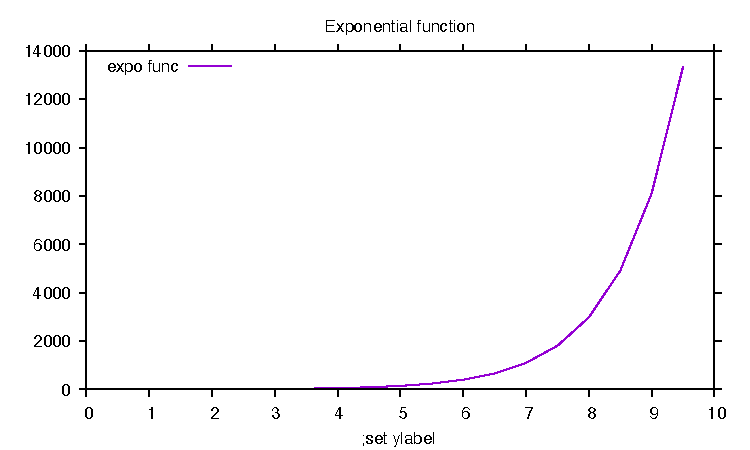
\includegraphics[width=0.75\textwidth]{expo.pdf}
%  \caption{The exponential function using the code above}
%  \label{Expo}
%\end{figure}
\begin{figure}[H]
  \centering
  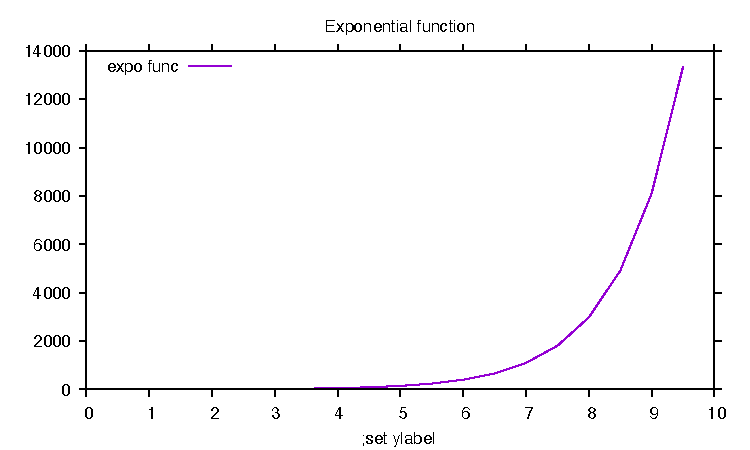
\includegraphics[width=0.75\textwidth]{expo}
  \caption{The exponential function using the code above}
  \label{Expo}
\end{figure}





\end{document}
